\documentclass[12pt,twoside]{article}
\usepackage{amsmath, amssymb}
\usepackage[active]{srcltx}
\usepackage{amssymb}
\usepackage{amscd}
\usepackage{makeidx}
\usepackage{amsthm}
\usepackage{algorithm}
\usepackage{algpseudocode}
\usepackage{wrapfig,lipsum}

\usepackage{fancyhdr}
\usepackage{graphics}
%----------------------------------------------------------------------------------------------
\usepackage{amsmath, amssymb}
\usepackage{amsmath}
\usepackage[active]{srcltx}
\usepackage{amssymb}
\usepackage{amscd}
\usepackage{makeidx}
\usepackage[dvips]{graphicx}
\usepackage{latexsym}

\renewcommand{\baselinestretch}{1}
\setcounter{page}{1}
\setlength{\textheight}{21.6cm}
\setlength{\textwidth}{14cm}
\setlength{\oddsidemargin}{1cm}
\setlength{\evensidemargin}{1cm}
\pagestyle{myheadings}
\thispagestyle{empty}
\markboth{\small{Pr\'actica 1. Anthony Steiner.}}{\small{.}}
\date{}
\begin{document}

\begin{figure}[h]
\vspace{-3cm} \hspace{-2cm} \setlength{\unitlength}{1mm}
\begin{picture}(15,25)(-10,0)

\includegraphics[width=16cm,height=3cm]{titulo.jpg}
\end{picture}
\end{figure}

\vspace{0cm}

\centerline{\bf An\'alisis de Algoritmos, Sem: 2022-2, 3CV11, Pr\'actica 1, 28/02/2022}

\centerline{}

%\centerline{}

\begin{center}
\Large{\textsc{Pr\'actica 1: Determinaci\'on experimental de la complejidad temporal de un algoritmo}}
\end{center}
\centerline{}
\centerline{\bf {Steiner V\'azquez Anthony Francis}}
\centerline{}
\centerline{$asteinerv1700@alumno.ipn.mx$}


\newtheorem{Theorem}{\quad Theorem}[section]

\newtheorem{Definition}[Theorem]{\quad Definition}

\newtheorem{Corollary}[Theorem]{\quad Corollary}

\newtheorem{Lemma}[Theorem]{\quad Lemma}

\newtheorem{Example}[Theorem]{\quad Example}

\bigskip

\textbf{Resumen:} En el presente trabajo se presentan 2 algoritmos, de los cuales veremos su funcionamiento, adem\'as, haremos un an\'alisis a posteriori, es decir, el an\'alisis experimental, de la complejidad temporal de dichos algoritmos. Esto se har\'a mediante el uso de un contador, en el c\'odigo implementado del algoritmo, para contar cada operaci\'on realizada por el algoritmo que se est\'e midiendo, 
m\'as tarde, mediante el uso de gr\'aficas obtendremos una representaci\'on del tiempo que tardan en ejecutarse dichos algoritmos. Para desarrollar cada gr\'afica, evaluaremos algunos puntos, y buscaremos una funci\'on que acote dichos puntos por arriba o, dependiendo del caso, por abajo.
Estas funciones ser\'an las funciones de complejidad temporal de los algoritmos.

{\bf Palabras Clave:} C++, Algoritmo, Complejidad, Tiempo

\section{Introducci\'on}
Esta pr\'actica fue realizada para presentar una manera de medir el tiempo que tarda en ejecutarse un algoritmo, y poder apreciar, de manera gr\'afica, el comportamiento de dichos algoritmos, en algunos casos particulares. Para ello necesitamos, primero, de un algoritmo el cual ser\'a medido; segundo, necesitamos checar cu\'al caso nos interesa, puede ser el mejor caso, el peor, o ambos;
tercero, implementar el algoritmo en alg\'un lenguaje de programaci\'on, en este caso se usar\'a C++; cuarto, agregaremos un contador al c\'odigo, con lo cual cada vez que se ejecute una l\'inea de c\'odigo sumaremos 1 a dicho contador, as\'i mediremos la cantidad de operaciones realizadas por el algoritmo; quinto y \'ultimo, graficaremos los puntos que se obtienen de la entrada y el n\'umero de operaciones ejecutadas, para encontrar la funci\'on que lo acote, dependiendo del caso, por ejemplo: para el mejor caso deber\'a acotarlo por abajo,
y para el peor caso, deber\'a acotarlo por arriba.

\newpage

Ahora, surgen las preguntas ¿Por qu\'e es importante un algoritmo? ¿Por qu\'e es importante analizar un algoritmo? Para responder a la primer pregunta, diremos que los algoritmos son parte importante de la computaci\'on, pr\'acticamente cualquier cosa en la computaci\'on fue diseñada e implementada por 1 o m\'as algoritmos, sean para software o para hardware, como por ejemplo las interfaces gr\'aficas, o un algoritmo para desarrollar hardware, y es por eso mismo que un algoritmo puede ser considerado como tecnolog\'ia, 
haciendo de su uso, algo cotidiano; a pesar de no ser implementados directamente por uno, pues cada dispositivo que ocupamos ocupa alguno en su n\'ucleo.
Para la segunda pregunta hay que ver que un algoritmo es una herramienta que nos permite resolver problemas, y esto nos lleva a considerar cu\'ales son mejores dependiendo de la memoria y el tiempo que ocupen en resolver dicho problema, esto nos lleva a tener algoritmos que no son correctos, o que simplemente no resuelven un problema de manera eficiente (Cormen, 2001).
\newline
Con esto podemos decir que un algoritmo es un procedimiento para realizar una tarea, o en otras palabras, un algoritmo debe resolver un problema bien especificado. Un problema algor\'itmico es dado mediante la descripci\'on de su conjunto de instancias, con las cuales trabajar\'a, entonces al correr el algoritmo con alguna de estas instancias, la salida debe ser la correcta. A esto le llamamos un algoritmo correcto, ahora bien, no basta con que un algoritmo sea correcto, tambi\'en debe ser eficiente (Skiena, 1998). Aunque ¿Por qu\'e es tan importante que un algoritmo sea eficiente? 
Lo veremos con un ejemplo: supongamos que tenemos un algoritmo que para una entrada n, ejecuta 100,000,000 de operaciones, y otro algoritmo que hace 1,000,000 de operaciones, y ejecutamos estos algoritmos en una computadora que realiza 1,000,000 de instrucciones por segundo. Aunque ambos resuelven el mismo problema, la computadora tardar\'ia 100 segundos en ejecutar el 1er algoritmo, mientras que solo 1 para el segundo. Si a esto le sumamos que los algoritmos son usados por grupos multidisciplinarios que resulven problemas, y deben hacerlo de la manera m\'as r\'apida, gastando la menor cantidad de recursos, podr\'iamos decir que
el segundo algoritmo es mejor que el primero, aunque hacerlo con este tipo de comparaciones no es lo ideal, nosotros buscaremos funciones que puedan describir el comportamiento, veremos que existen familias de funciones que describen comportamientos similares entre los algoritmos que pueden o no, resolver el mismo problema (Cormen, 2001).
\newline
As\'i, el objetivo de esta pr\'actica es mostrar el funcionamiento de 2 algoritmos que resuelven 2 problemas diferentes, para medir el tiempo que tardan en realizar esta tarea de manera correcta y adem\'as darnos una idea de si son eficientes. Finalmente observaremos que el tiempo que tardan en ejecutarse estos algoritmos puede ser acotado por alguna funci\'on que dicta el comportamiento del algoritmo, separandolo por casos, para darnos una mejor idea de cu\'anto debe tardar en ejecutarse el algoritmo que estamos ocupando.

\section{Conceptos B\'asicos}

Una funci\'on $\mathnormal{f}$ es una correspondencia que mapea un elemento $\mathnormal{x}$ de un conjunto $\mathit{D}$, el dominio de la funci\'on, a un \'unico elemento $\mathnormal{f}$($\mathnormal{x}$) de un conjunto $\mathit{E}$, el rango de la funci\'on. Un m\'etodo para visualizar una funci\'on, es a trav\'es de su gr\'afica, esto es, el conjunto de parejas ordenadas \{ ($\mathnormal{x}$,$\mathnormal{f}$($\mathnormal{x}$)) $\mid$ $\mathnormal{x}$ $\in$ $\mathit{D}$ \}.
\newline
\newline
Un problema $\mathit{P}$ es una funci\'on cuyo dominio es un conjunto de instancias $\mathit{I}$, y como contradominio(rango), un conjunto de soluciones $\mathit{S}$ i.e.\ $\mathit{P}$ : $\mathit{I}$ $\to$ $\mathit{S}$. Las instancias son una entrada en particular para el problema. 
\newline
\newline
Un algoritmo es una secuencia ordenada de pasos para resolver un problema, este debe ser preciso, es decir, tiene pasos definidos de manera clara; debe ser finito, esto es, que termina en alg\'un momento; y finalmente debe estar definido, lo que nos garantiza que siguiendo los pasos, se llega a la misma salida siempre. Estos se representan generalmente con pseudo-c\'odigo.
\newline
Si dado un problema $\mathit{P}$ existe un algoritmo $\mathit{A}$ de tal manera que para cada elemento $\mathnormal{x}$ $\in$ $\mathit{I}$, $\mathit{A}$ produce como salida el elemento $\mathit{P}$($\mathnormal{x}$) $\in$ $\mathit{S}$ entonces se dice que $\mathit{P}$ es computable i.e.\
$\mathit{P} : \mathit{I} \to \mathit{S}, \exists \mathit{A} \mid \forall \mathnormal{x} \in \mathit{I}, \mathit{A}(\mathnormal{x}) = \mathit{P}(\mathnormal{x}) \in \mathit{S} \to \mathit{P}$ es computable. Los problemas que se pueden resolver en una computadora son el conjunto de problemas computables.
\newline
\newline
Un algoritmo es correcto, si para cada instancia de entrada, el algoritmo se detiene con la salida correcta, en tal caso, decimos que el algoritmo resuelve el problema. Un algoritmo es eficiente cuando resuelve el problema con la menor cantidad de recursos, como por ejemplo el tiempo que tarda en ejecutarse, entonces podemos encontrar una funci\'on que nos diga el n\'umero de operaciones o pasos a ejecutar por un algoritmo para resolver un problema con una entrada de tamaño $\mathnormal{n}$. Se denota por $\mathit{T}(\mathnormal{n})$, y se le conoce como funci\'on de complejidad temporal del algoritmo.
\newline
\newline
Al c\'alculo experimental en la que se recogen datos estad\'isticos del tiempo consumido por el algoritmo mientras se ejecuta en una computadora en particular, se le conoce como an\'alisis a $\mathit{posteriori}$.
\newline
\newline
Despu\'es de hacer el an\'alisis a $\mathit{posteriori}$ de un algoritmo, obtendremos la funci\'on de complejidad temporal $\mathit{T}(\mathnormal{n})$, la cual se puede acotar por arriba, y por abajo con alguna funci\'on, lo cual nos da una idea del orden de crecimiento de la funci\'on de complejidad, adem\'as, nos permite tener una carecterizaci\'on simple de la eficiencia de un algoritmo, y tambi\'en nos permite comparar el rendimiento de los algoritmos. A esto se le conoce como eficiencia asint\'otica de un algoritmo, y tenemos las siguientes notaciones:
\newline
$\Theta(\mathit{g}(\mathnormal{n})) = \{ \mathnormal{f}(\mathnormal{n}) : \exists \mathnormal{n}$  $c_1,c_2 > 0 $ \& $ n_0>0 \mid 0 \le c_1\mathnormal{g}(\mathnormal{n}) \le \mathnormal{f}(\mathnormal{n}) \le c_2 \mathnormal{g}(\mathnormal{n})$ $ \forall n \ge n_0 \}$. Esto significa que $ \mathnormal{f}(\mathnormal{n})$ est\'a acotada por arriba y por abajo por $\mathnormal{g}(\mathnormal{n})$ y esto se cumple para toda $\mathnormal{n} \ge n_0$. Es decir $\mathnormal{g}(\mathnormal{n})$ es un ajuste asint\'otico para $\mathnormal{f}(\mathnormal{n})$.
\newline
\newline
$O(\mathit{g}(\mathnormal{n})) = \{ \mathnormal{f}(\mathnormal{n}) : \exists \mathnormal{n}$  $c > 0 $ \& $ n_0>0 \mid 0 \le \mathnormal{f}(\mathnormal{n}) \le c \mathnormal{g}(\mathnormal{n})$ $ \forall n \ge n_0 \}$. Es decir $g(n)$ es un ajuste asint\'otico superior para $f(n)$. Se usa para denotar el peor caso de un algoritmo, es decir cuando hace la mayor cantidad de operaciones.
\newline
\newline
$\Omega(\mathit{g}(\mathnormal{n})) = \{ \mathnormal{f}(\mathnormal{n}) : \exists \mathnormal{n}$  $c > 0 $ \& $ n_0>0 \mid 0 \le c \mathnormal{g}(\mathnormal{n}) \le \mathnormal{f}(\mathnormal{n}) $ $ \forall n \ge n_0 \}$. Es decir $g(n)$ es un ajuste asint\'otico inferior para $f(n)$. Se usa para denotar el mejor caso de un algoritmo, es decir cuando hace la menor cantidad de operaciones.
\newline
\newline
Si tenemos 2 funciones $f(n)$ y $g(n)$, $f(n) \in \Theta(g(n)) \Longleftrightarrow f(n) \in O(g(n))$ y $f(n) \in \Omega(g(n))$. 
\newline
\newline
Ya que estas notaciones son conjuntos podr\'iamos escribir $f(n) \in \Theta(g(n))$ para indicar que $f(n)$ es un miembro de $\Theta(g(n))$. Aunque tambi\'en podr\'iamos escribir $f(n) = \Theta(g(n))$ para expresar la misma noci\'on.
\newline
\newline
Para darnos una idea de c\'omo se usan estas notaciones haremos una analog\'ia entre la comparaci\'on asint\'otica de 2 funciones $f$ y $g$, y la comparaci\'on de 2 n\'umeros reales $a$ y $b$:
\newline
$f(n) = O(g(n))$ es como $a \le b$,
\newline
$f(n) = \Omega(g(n))$ es como $a \ge b$,
\newline
$f(n) = \Theta(g(n))$ es como $a = b$.
\newline
\newline
Los algoritmos que se presentan en este trabajo son los siguientes:
\newline
\newline
1) Algoritmo de b\'usqueda en sub-arreglos 
\newline
Este algoritmo checa si para un arreglo dado, existe un elemento igual en los subarreglos que se formar\'ian de partir a la mitad el arreglo, y si existe un elemento as\'i, muestra cu\'al fue ese elemento, y sus posiciones en el arreglo, en caso de que no exista, simplemente se detiene.
\newline
\newline
2) Algoritmo de Euclides
\newline
Este algoritmo calcula el m\'aximo com\'un divisor de 2 n\'umeros enteros positivos, mediante el m\'etodo de divisiones.
\newline
\newline
A continuaci\'on veremos sus pseudo-c\'odigos:
\begin{algorithm}
    \caption{BusquedaEnSubArreglo($arr$):}
    \begin{algorithmic}
    \State $tam \gets arr.size()$
    \State $valor \gets -1$
    \State $posi \gets -1$
    \State $posf \gets -1$
    \If{$arr[0] = arr[tam/2]$}
        \State $valor \gets arr$
        \State $posi \gets 0$
        \State $posf \gets tam/2$
    \Else
        \State $hashtam \gets hash.size()$
        \For{$i = 0$ \textbf{to} $i < hashtam$ }
            \State $hash[i] \gets -1$
        \EndFor
        \For{$i = 0$ \textbf{to} $i < tam$ } 
            \If{$i < tam$}
                \State $hash[arr[i]] \gets arr[i]$
            \Else
                \If{$hash[arr[i]] \neq -1$}
                    \State $valor \gets arr[i]$
                    \State $posf \gets i$
                    \State \textbf{break}
                \EndIf
            \EndIf
        \EndFor
        \For{$i = 0$ \textbf{to} $i < tam/2$ }
            \If{ $arr[i] = valor$}
                \State $posi \gets i$
                \State \textbf{break}
            \EndIf
        \EndFor
        \If{$valor \neq -1 \&\& posi \neq -1 \&\& posf \neq -1$}
            \State $print(*)$
        \EndIf
    \EndIf 
    \end{algorithmic}
\end{algorithm}
\newpage
\begin{algorithm}
    \caption{AlgoritmoDeEuclides($m$, $n$) :}
    \begin{algorithmic}
    \While{$n \neq 0$}
    \State $r \gets m$ $mod$ $n$
    \State $m \gets n$
    \State $n \gets r$
    \EndWhile
    \State \textbf{return} $m$
    \end{algorithmic}
\end{algorithm}

Ahora veremos su funcionamiento dando unos ejemplos de instancias:
\newline
Para el algoritmo de B\'usquedaEnSubArreglo daremos como instancia el arreglo $A[4,5,0,9,4,1,2,5,3,0]$ y la soluci\'on es que el valor repetido en los subarreglos $A[0,..., n/2] $ y $A[n/2 + 1, ..., n-1]$ es 5, en las posiciones $[1]$ y $[7]$.
El algoritmo guarda en $tam$ el valor del tamaño del arreglo e inicializa las variables $valor$, $posi$ y $posf$ con -1. Checa si el valor del primer subarreglo es el mismo que el del segundo subarreglo, esto ser\'ia el mejor caso, de ser as\'i, actualiza los valores de las variables $valor$, $posi$ y $posf$; ya que no es el caso entonces creamos un arreglo auxiliar y en la variable $hashtam$ guardamos el valor de su tamaño, ya que este arreglo ser\'a usado para hashear debe ser suficientemente grande, es decir, debe tener como tamaño el valor m\'aximo contenido en nuestro arreglo original, como m\'inimo; ya que usaremos la funci\'on de hasheo identidad, es decir guardaremos el valor de nuestro arreglo original en la posici\'on que sea igual a ese valor, y por tanto primero debemos inicializar todos sus elementos con -1.
Luego itera sobre nuestro arreglo original y checa si estamos en la primera mitad, de ser as\'i, hashea los elementos, ya en la 2nda mitad checa si ese valor ya fue hasheado, pues esto quiere decir que encontramos un valor repetido, entonces actualizaremos las variables $valor$ y $posf$, y romperemos el ciclo. Aunque nos falta encontrar el valor de $posi$, as\'i que volveremos a iterar sobre nuestro arreglo pero esta vez solo en la primera mitad, y en el momento que encontremos el valor, actualizamos el valor de $posi$, y romperemos el ciclo.
Finalmente si se ha encontrado un elemento en ambos subarreglos, lo muestra en pantalla, de lo contrario, simplemente se detiene.
\newline
\newline
Por otro lado el algoritmo de Euclides entra en un ciclo hasta que nuestra variable $n$ sea 0, 
posteriormente guarda en una variable $r$ el residuo de la divisi\'on entre $m$ y $n$, y despu\'es guarda el nuevo $m$ que ser\'a $n$, y el nuevo $n$, que ser\'a $r$, es decir el residuo que ya hab\'iamos calculado anteriormente, de esta manera siempre estaremos calculando el modulo, del modulo, y as\'i sucesivamente desde la primera divisi\'on hasta que nuestra $n$, que fue el \'ultimo modulo, nos de 0, de tal manera en $m$ habremos guardado el valor de nuestro m\'aximo com\'un divisor, que para el peor caso se trata de los primos relativos, que se dan en valores consecutivos de la sucesi\'on de Fibonacci, es decir 2 n\'umeros cuyo m\'aximo com\'un divisor $mcd(m,n) = 1$.
\newpage

Por ejemplo con la intancia $m=34$, $n=21$, la soluci\'on es 1, puesto que son primos relativos. Por lo tanto el algoritmo empieza en un ciclo donde inicilamente $r=0$, $m=34$, y $n=21$; en la 1ra iteraci\'on $r=13$, $m=21$, y $n=13$, en la 2nda iteraci\'on $r=8$, $m=13$, $n=8$, en la 3ra iteraci\'on $r=5$, $m=8$, y $n=5$, en la 4ta iteraci\'on $r=3$, $m=5$, y $n=3$, en la 5ta iteraci\'on $r=2$, $m=3$ y $n=2$, en la 6ta iteraci\'on $r=1$, $m=2$, y $n=1$, y por \'ultimo en la 7ma iteraci\'on $r=0$, $m=1$, y $n=0$, por lo tanto deja de iterar, y nuestro $mcd$ es igual a 1, recordemos que el m\'aximo com\'un divisor, es el n\'umero m\'as grande que divide a ambos n\'umeros sin dejar residuo.
\newline
\newline 
Podemos observar que ambos algoritmos son correctos, así que procedemos a checar su eficiencia, haciendo un análisis a $posteriori$ de los mismos.

\section{Experimentaci\'on y Resultados}

Para nuestro primer algoritmo el tamaño del problema es el tamaño del arreglo donde buscaremos al elemento en los subarreglos. Así que checaremos cu\'antas operaciones realiza nuestro algoritmo dependiendo del valor de $tam$, al que vamos a restringir a n\'umeros pares, tanto para el mejor caso, como para el peor caso; como previamente discutimos, el mejor caso se encuentra cuando el valor en la primera posición de ambos subarreglos es igual, sin embargo, para poder definir cu\'al es el peor caso deberemos de checar m\'as a detalle la implementaci\'on del algoritmo, puesto que existe la opci\'on de que el peor caso sea que no exista un elemento que cumpla que est\'e en ambos subarreglos, sin embargo,
tambi\'en puede ser que el peor caso, sea cuando el valor que se repite est\'a en las últimas posiciones de los subarreglos. Así que nos apoyaremos del an\'alisis a $posteriori$ para determinar cu\'al es el peor caso, y adem\'as saber cu\'al es la funci\'on que lo acota, es decir, su funci\'on de complejidad temporal.
\newline
\newline
Para el segundo algoritmo definiremos como tamaño del problema a nuestro n\'umero $m$, ya que en particular para el peor caso estaremos checando n\'umeros consecutivos de la sucesi\'on de Fibonacci, de tal manera que m ser\'a el mayor de estos 2 n\'umeros, y vamos a checar cu\'antas operaciones realiza dadas estas condiciones.
\newline
\newline
Ahora pasaremos a ejecutar nuestros algoritmos, y contar el n\'umero de operaciones que ejecuta para realizar su tarea correctamente, para ello hemos agregado al c\'odigo en C++ un contador, que aumentara por cada operaci\'on realizada por el algoritmo. As\'i bien procedemos a ejecutar nuestro primer algoritmo y analizar su comportamiento tanto en el mejor como en el peor caso.
\newpage
Empezaremos con nuestro algoritmo de b\'usqueda en subarreglos.
\begin{figure}[h]
\vspace{3cm} \hspace{-2cm} \setlength{\unitlength}{1mm}
    \begin{picture}(15,25)(-35,0)
        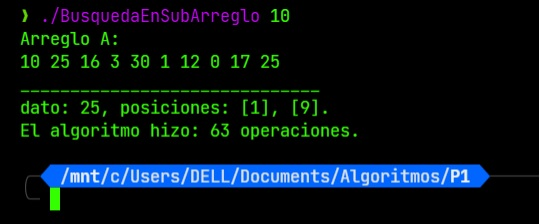
\includegraphics[width=10cm,height=5cm]{subarray_run.jpg}
    \end{picture}
\end{figure}
\vspace{-1cm}
\begin{center}
    Figura 1. Ejecuci\'on del c\'odigo de B\'usqueda en subarreglo.
\end{center}
\medskip
Para analizar a $posteriori$ un algoritmo iremos aumentando el valor de $n$ que es el tamaño del problema, entonces procedemos a ejecutar nuestro c\'odigo aumentando de 10 en 10 el tamaño del arreglo que se guarda en $tam$ puesto que esa es nuestra $n$, para obtener varias mediciones.
\newline
\newline
As\'i para el mejor caso tenemos:
\begin{table}[htbp]
    \begin{center}
        \begin{tabular}{|c|c|}
            \hline
            \textbf{m} & \textbf{\# operaciones} \\
            \hline \hline
            10 &	11 \\ \hline
            20 &11 \\ \hline
            30 &	11 \\ \hline
            40 &	11 \\ \hline
            50 &	11 \\ \hline
            60 &	11 \\ \hline
            70 & 11 \\ \hline
            80 & 11 \\ \hline
            90 & 11 \\ \hline
            100 & 11 \\ \hline
        \end{tabular}
        \caption{Mediciones para el mejor caso de B\'usqueda en subarreglo}
        \label{tabla:analisis1}
    \end{center}
\end{table}
\medskip
\newline
Desp\'ues, para determinar el peor caso, se tuvieron que hacer mediciones para cuando se encuntran valores que cumplan las condiciones y para cuando no se cumple.
\newpage
As\'i para el caso en que se encuntran los valores:
\begin{table}[htbp]
    \begin{center}
        \begin{tabular}{|c|c|}
            \hline
            \textbf{m} & \textbf{\# operaciones} \\
            \hline \hline
            10 &	55 \\ \hline
            20 &	86 \\ \hline
            30 &	178 \\ \hline
            40 &	221 \\ \hline
            50 &	152 \\ \hline
            60 &	196 \\ \hline
            70 & 269 \\ \hline
            80 & 318 \\ \hline
            90 & 345 \\ \hline
            100 & 366 \\ \hline
        \end{tabular}
        \caption{Mediciones para el caso en que se encuntran valores iguales}
        \label{tabla:analisis2}
    \end{center}
\end{table}
\newline
Ahora para cuando no se encuntran los valores:
\begin{table}[htbp]
    \begin{center}
        \begin{tabular}{|c|c|}
            \hline
            \textbf{m} & \textbf{\# operaciones} \\
            \hline \hline
            10 &	67 \\ \hline
            20 &	122 \\ \hline
            30 &	177 \\ \hline
            40 &	232 \\ \hline
            50 &	287 \\ \hline
            60 &	342 \\ \hline
            70 & 397 \\ \hline
            80 & 452 \\ \hline
            90 & 507 \\ \hline
            100 & 562 \\ \hline
        \end{tabular}
        \caption{Mediciones para el caso en que no se encontraron valores iguales}
        \label{tabla:analisis3}
    \end{center}
\end{table}
\newline
As\'i podemos observar que el peor caso es cuando no existen valores iguales en los subarreglos.
\newline
Con esta informaci\'on vamos a proponer funciones que pasen por la mayor cantidad de puntos, o que los acoten, y diremos que esa es su $T(n)$, para posteriormente graficar el n\'umero de operaciones v.s.\ $n$.
\newline
\newline
Para el mejor caso, propondremos la funci\'on $f(n) = 10$, y para el peor caso proponemos $f(n) = 7n$.
\newpage
\begin{figure}[h]
    \vspace{3cm} \hspace{-2cm} \setlength{\unitlength}{1mm}
        \begin{picture}(15,25)(-35,0)
            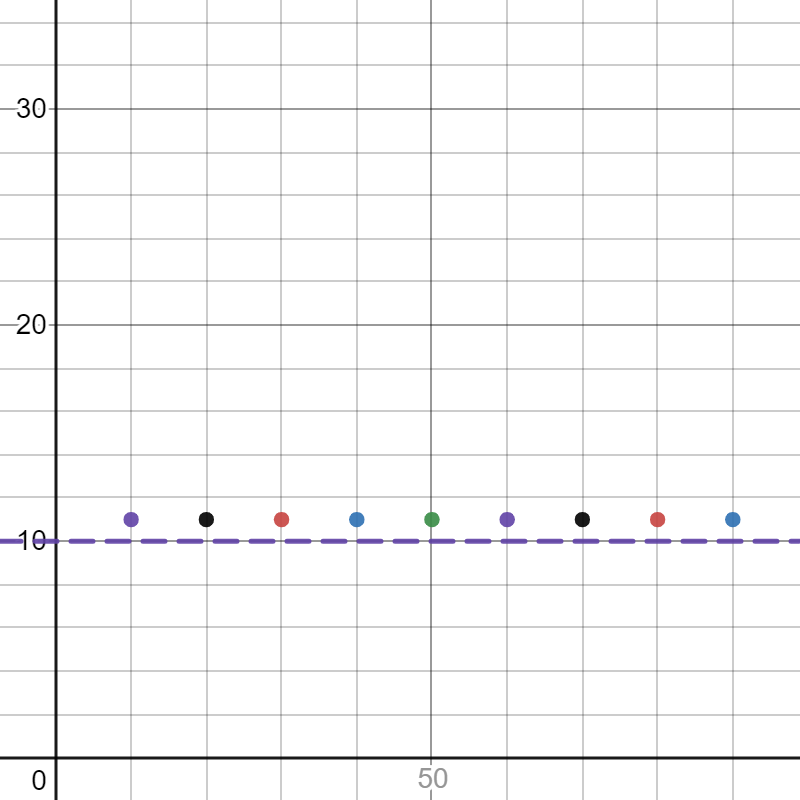
\includegraphics[width=10cm,height=5cm]{subarreglo_mc.png}
        \end{picture}
    \end{figure}
    \vspace{-1cm}
    \begin{center}
        Figura 2. Gr\'afica de la funci\'on $f(n) = 10$
    \end{center}
    \medskip
Ya que todos los puntos quedan por encima de la funci\'on $f(n) = 10$ podemos decir que la $T(n)$ para el mejor caso de  BusquedaEnSubArreglo, es: $f(n) = 11 \in \Omega(1)$.

\begin{figure}[h]
    \vspace{3cm} \hspace{-2cm} \setlength{\unitlength}{1mm}
        \begin{picture}(15,25)(-35,0)
            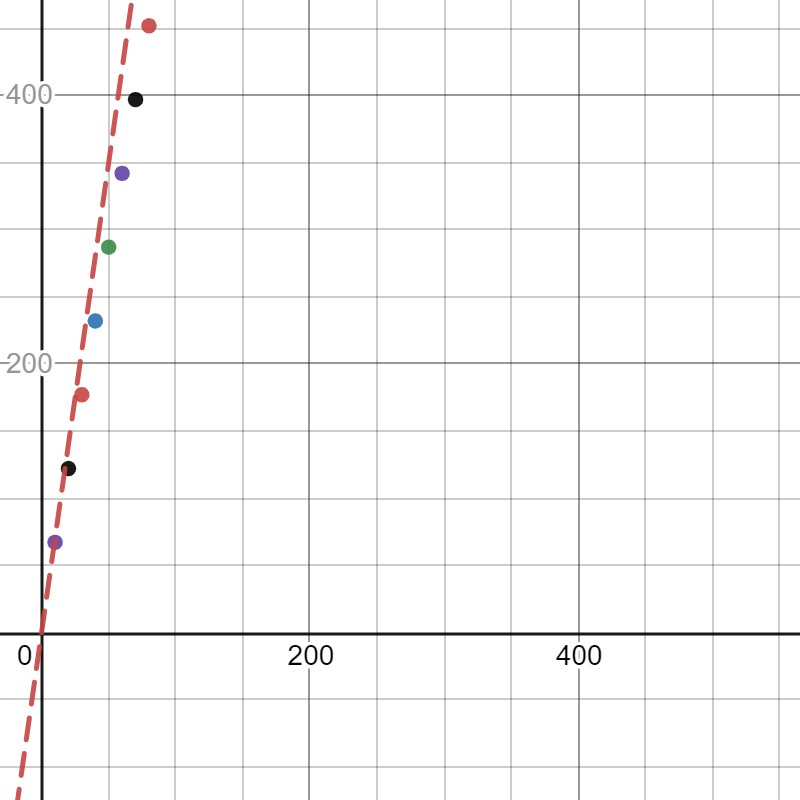
\includegraphics[width=10cm,height=5cm]{subarray_wc.png}
        \end{picture}
    \end{figure}
    \vspace{-1cm}
    \begin{center}
        Figura 3. Gr\'afica de la funci\'on $f(n) = 7n$
    \end{center}
    \medskip
Ya que todos los puntos quedan por debajo de la funci\'on $f(n) = 7n$ podemos decir que la $T(n)$ para el peor caso de  BusquedaEnSubArreglo, es: $f(n) = 7n \in O(n)$.
\newpage
Por \'ultimo veremos el funcionamiento del algoritmo de Euclides:
\begin{figure}[h]
    \vspace{3cm} \hspace{-2cm} \setlength{\unitlength}{1mm}
        \begin{picture}(15,25)(-35,0)
            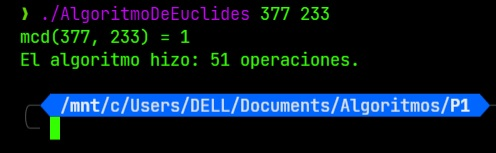
\includegraphics[width=10cm,height=5cm]{euclides_run.jpg}
        \end{picture}
    \end{figure}
    \vspace{-1cm}
    \begin{center}
        Figura 4. Ejecuci\'on del c\'odigo para Euclides.
    \end{center}
    \medskip
Ahora analizaremos los resultados experimentales arrojados por el algoritmo de Euclides, para el peor caso:
\begin{table}[htbp]
    \begin{center}
        \begin{tabular}{|c|c|}
            \hline
            \textbf{m} & \textbf{\# operaciones} \\
            \hline \hline
            1 &	7 \\ \hline
            2 &	7 \\ \hline
            3 &	11 \\ \hline
            5 &	15 \\ \hline
            8 &	19 \\ \hline
            13 &	23 \\ \hline
            21 & 27 \\ \hline
            34 & 31 \\ \hline
            55 & 35 \\ \hline
            89 & 39 \\ \hline
            144 & 43 \\ \hline
        \end{tabular}
        \caption{Mediciones para el peor caso de Euclides}
        \label{tabla:analisis4}
    \end{center}
\end{table}

Para el peor caso de euclides proponemos la funci\'on $f(n) = 18 log_2(n)$.
\newpage
\begin{figure}[h]
    \vspace{3cm} \hspace{-2cm} \setlength{\unitlength}{1mm}
        \begin{picture}(15,25)(-35,0)
            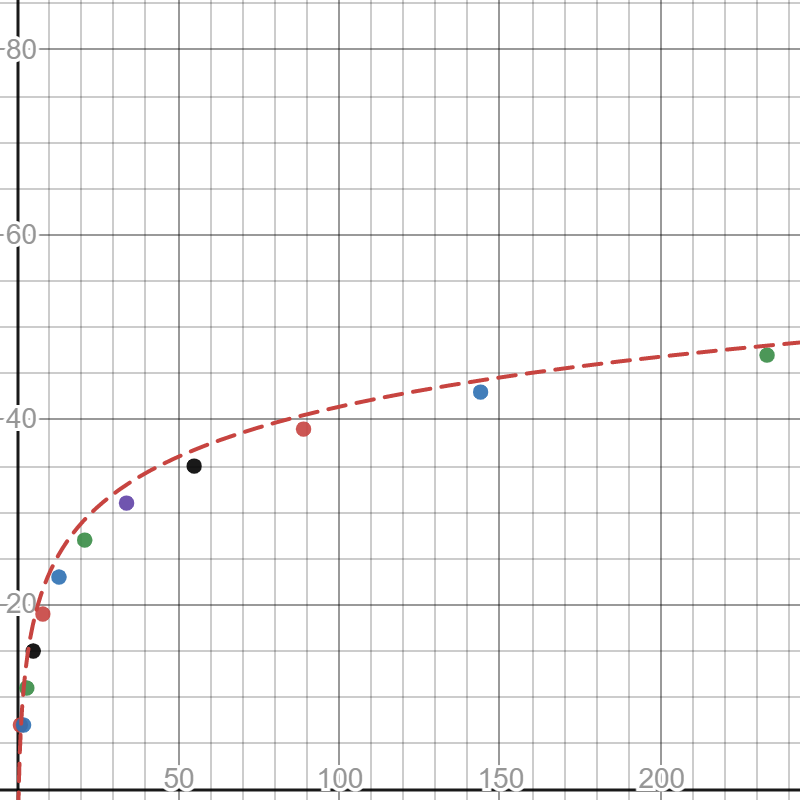
\includegraphics[width=10cm,height=5cm]{Euclides-plot.png}
        \end{picture}
    \end{figure}
    \vspace{-1cm}
    \begin{center}
        Figura 5. Gr\'afica de la funci\'on $f(n) = 18 log_2(n)$
    \end{center}
    \medskip
    Ya que todos los puntos quedan por debajo de la funci\'on $f(n) = 18log_2(n)$ podemos decir que la $T(n)$ para el peor caso del algoritmo de Euclides, es: $f(n) = 18 log_2(n) \in O(nlog(n))$.

\section{Conclusiones}
\textbf{Conclusi\'on General}
\newline
Para esta pr\'actica uno de los problemas que se present\'o fue que el algoritmo inicialmente planteado para el 1er problema era de complejidad cuadr\'atica, debido a esto, un an\'alisis m\'as completo fue necesario para poder tener una mejor complejidad, para ello fue necesario checar si un mapeo hash resolv\'ia el problema, y de esto surgi\'o el problema de encontrar una funci\'on hash 
que se adecuara a nuestra situaci\'on, as\'i que se opt\'o por la funci\'on hash de identidad, aunque esta funciona bien solo para valores pequeños, as\'i que quiz\'as una manera de poder mejorar este algoritmo ser\'ia el de implementar una mejor funci\'on hash, que sea m\'as general, aunque independientemente de eso, pudimos observar que nuestro algoritmo es correcto, por lo tanto se tuvieron los 
resultados esperados, y ahora con una complejidad lineal, as\'i que se logr\'o mejorar la eficiencia del algoritmo; aunque es posible que para cuando no se encuntren valores repetidos en los subarreglos, se podr\'ia a\'un mejorar la cantidad de operaciones, pero seguir\'ia siendo lineal. Otra duda que surgi\'o era el qu\'e suced\'ia si nuestro algoritmo no encontraba un elemento con las caracter\'isticas que nos solicitaban, as\'i que se opt\'o por inicializar todas nuestras variables auxiliares con -1, y si no se modificaban, entonces simplemente no mostraba nada, pero se deten\'ia de todos modos.
Para el segundo algoritmo surgieron dudas de realmente cu\'al era la funci\'on que acotaba por arriba nuestros puntos, pero despu\'es de analizar puntos fuera del peor caso, y checar m\'as puntos, nos dimos cuenta de que la funci\'on ten\'ia un comportamiento parecido al logar\'itmico.
\newpage
\textbf{Conclusi\'on de Anthony}

\begin{wrapfigure}{r}{5.5cm}

\includegraphics[width=5.5cm]{me.jpg}
\end{wrapfigure} 

En particular de los algoritmos que se checaron en esta pr\'actica, del 1ro me llam\'o mucho la atenci\'on el 
poder analizar un algoritmo que aunque ya es correcto, no quedas satisfecho con su desempeño, y por lo tanto regresar a la fase de diseñar el algoritmo, y checar como optimizarlo, fue muy interesante. Además de poder pensarlo en casos, tambi\'en ayud\'o a quitar complejidad innecesaria del algoritmo. Del segundo algoritmo, me llam\'o mucho la atenci\'on que justo el peor caso para calcular el mcd de 2 n\'umeros sea cuando cumplan la propiedad de que sean primos relativos, y que justo 2
n\'umeros consecutivos de la sucesi\'on de Fibonacci cumplan esta propiedad, me pareci\'io incre\'ible.

\section{Anexo}
Para este caso no se realizaron problemas de tarea para anexar.

\section{Bibliograf\'ia}

Cormen, T. H., \& Cormen, T. H. (2001). Introduction to algorithms. Cambridge, Mass: MIT Press.
\newline
Skiena, S. S. (1998). The algorithm design manual. New York: Springger-Verlang.
\medskip

\end{document}